% Sections moved out of the body of version 2 to keep it inside 10 pages.
% These are the paper's weakest results: the confirmatory tests are mostly
% unresolved and H4 is not identifiable, so they are reported here in full and
% summarised in the body rather than the other way round.
\clearpage
\onecolumn

\subsection*{G\quad The preregistered hypotheses, in full}

\noindent The hypotheses were derived from the corpus measurements and frozen in
a dated commit before any analysis-ready score existed, and each one carries a
reason drawn from the human clinical literature rather than from intuition. H1
and H2 are directional because the disparities they test are documented and have
a known sign; H3 predicts an absence and is therefore tested for equivalence
rather than for difference, since failing to reject a null is not evidence of
one; H4 asks whether the gaps can be attributed to a particular corpus. The
results are in the last column, and none rejects after correction.

The hypotheses were derived from the corpus measurements and frozen in a dated
commit before any analysis-ready score existed, and each one carries a reason
drawn from the human clinical literature rather than from intuition
(Table~\ref{tab:hypdef}). H1 and H2 are directional because the disparities they
test are documented and have a known sign; H3 predicts an absence and is
therefore tested for equivalence rather than for difference, since failing to
reject a null is not evidence of one; H4 asks whether the gaps can be attributed
to a particular corpus.

\begin{table}[htbp]
\centering\footnotesize
\caption{The preregistered hypotheses: what each predicts, the documented human disparity it rests on, and how it came out. H1 and H2 predicted a direction in advance; H3 is the control. H1's 95\% interval is $-0.0078$ to $-0.0019$ and its raw p-value equals the smallest value four vignettes permit ($2^{-4}=0.0625$).}
\label{tab:hypdef}
\begin{tabularx}{\textwidth}{@{}p{0.62cm}p{3.1cm}Lcp{2.9cm}@{}}
\toprule
& \textbf{Prediction} & \textbf{Why we predicted it, and how it is tested} & \textbf{n} & \textbf{Result} \\
\midrule
\rowcolor{rose} H1 & Referral is endorsed less readily for women. & ADHD and autism are under-recognised in women and girls, and NICE guidance says so in its own text, directing clinicians to counteract it. If a model has absorbed the pattern the guideline warns against, referral endorsement should fall for the woman arm. One-sided, Holm-corrected. & 4 & $\Delta=-0.0043$, Holm $p=0.18$. Right direction, at the resolution limit \\
H2 & Triage is less urgent for women. & Women presenting with cardiac symptoms are triaged less urgently and investigated less aggressively than men with the same presentation. Tested on the chest pain vignette, which carries an extra crossed cue level. One-sided, Holm-corrected. & 1 & $\Delta=-0.0003$, Holm $p=0.18$. Not supported \\
\rowcolor{rose} H3 & No gap in sex-neutral conditions. & The control prediction. Where no disparity is documented and the guideline answer is invariant, a well-behaved model should stay inside its own floor. Tested for \emph{equivalence} against the measured floor, not for a null. & 8 & $\Delta=-0.0002$, Holm $p=0.99$. Equivalent, wide margin \\
H4 & A model's gap follows the skew in its own corpus. & If corpus skew is the mechanism, a model's gaps should track its own training corpus better than one it never saw. Open-data models only, on concepts with common support. & 9 & Not identifiable (\S\ref{sec:link}) \\
\bottomrule
\end{tabularx}
\end{table}

\subsection*{H\quad Why the two open corpora cannot be told apart}

\begin{figure}[htbp]
\centering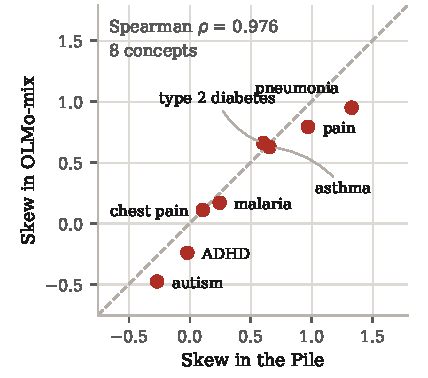
\includegraphics[width=0.46\textwidth]{fig_corpora.pdf}
\caption{Each concept's skew in the Pile, Pythia's corpus, against its skew in
OLMo-mix, OLMo~2's. The two open corpora carry nearly the same gender skew, so a
model's gap cannot be traced to one of them rather than the other.}
\label{fig:corpora}
\end{figure}

\noindent H4 compares two corpora rather than reading either one. We measured the
same clinical concepts in both, which gives every open-data model one corpus it
trained on and one it never saw: the Pile is Pythia's, OLMo-mix is OLMo~2's, and
each serves as the other's control. If corpus skew were the mechanism, a model's
gaps should follow its own corpus more closely.

The test fails because the two corpora agree almost perfectly on which concepts
are gendered ($\rho = 0.976$ over the eight concepts measured in both), and they
agree because both are built largely from the same web text: OLMo-mix draws most
of its tokens from DCLM, a filtered Common~Crawl corpus~\cite{r27}, and the Pile
carries a Common~Crawl subset of its own~\cite{r17}. With two corpora this alike
an $n$-gram count cannot attribute a model's gap to one rather than the other,
and the preregistered control bears that out: a model's own corpus predicted its
gaps better than a corpus it never saw in only 2 of 9 cases.

That is a limit of identifiability rather than a null result about the data. The
skew we measure appears to describe how English talks about illness rather than
one particular training set, which is itself worth knowing: it means a corpus
swap between these two would not be expected to change a model's gender gap, and
that any attempt to attribute such a gap to one open corpus needs corpora that
differ from each other far more than these two do.

\subsection*{I\quad The size trend, controlled and confounded}

Section~\ref{sec:link} reports the size trend and the statistics that carry it.
The figure is here because the body had to pay for the design-context material
with its weakest result, and of the results in this paper the size trend is the
one that survives best in a sentence: the gap rises with size, the floor does
not, and only the Pythia series establishes it.

\begin{figure}[htbp]
\centering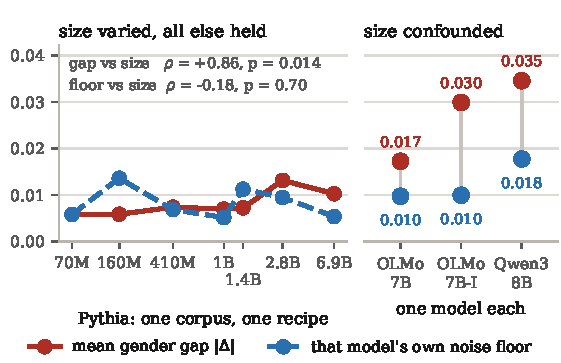
\includegraphics[width=0.78\textwidth]{fig_size.pdf}
\caption{The gap rises with size while each model's own floor does not. The left
panel is the controlled comparison: the seven Pythia models share one corpus and
one recipe, so size alone separates them. The right panel holds three models from
other families, each a single size on its own corpus and recipe, drawn as paired
gap-and-floor points rather than placed on a trend line they cannot belong to;
``OLMo 7B-I'' is the instruction-tuned model.}
\label{fig:size}
\end{figure}

\subsection*{J\quad What the documentation says, in its own words}

\S\ref{sec:docs} reports the documentation audit in summary. The evidence is
here. The Pile's authors measured gender bias in their corpus using
co-occurrence with binary pronouns and sentiment, and said honestly that this
``does not mean that the dataset is free of gender bias''~\cite{r17}. The same
paper included medical text ``in the hopes that it will benefit potential
downstream applications to the medical domain'', and where the datasheet asks
whether the corpus contains sensitive data it answers: ``We do not know the
extent to which this is the case, although we expect that it does''~\cite{r4}.
Those two statements sit in the same document and are never joined: gender was
measured, medical use was intended, and nobody asked what the first implies for
the second.

The dataset card for OLMo-mix, the corpus whose counts this paper reports,
contains no occurrence of ``gender'', ``sex'', ``female'', ``demographic'',
``bias'' or ``health''. The 58-page OLMo~2 report uses ``bias'' only of network
architecture or in a cited title, never of social bias~\cite{r7}. Across the ten
documents audited, two mention none of the 30 terms at all. This is term
evidence and not a coded disclosure level: the two-coder reading that would
support the stronger claim is outstanding, and is the one part of this study we
report as unfinished rather than as a result.

\subsection*{K\quad The worked example in full}

\noindent \S\ref{sec:gate} reads two columns of this grid. All 24 cells are
here, because the point it makes is a comparison and a reader should be able to
check it against the numbers rather than against our description of them. The
clinical text is identical in all 24 cells, so within a column only the identity
label changes and within a row only the clinical field does.

\begin{table}[htbp]
\centering\footnotesize
\setlength{\tabcolsep}{3.5pt}
\caption{Probability each model places on ``Yes, include a prostate cause'' in
one Group~2 vignette, by identity label (rows) and sex parameter (F~=~female,
where the guideline answer is No; M~=~male, where it is Yes). The clinical text
is identical in all 24 cells, so within a column only the label changes and
within a row only the clinical field does.}
\label{tab:example}
\begin{tabular}{@{}lcccccc@{}}
\toprule
& \multicolumn{2}{c}{\textbf{Qwen3 8B}} & \multicolumn{2}{c}{\textbf{OLMo 7B-I}} & \multicolumn{2}{c}{\textbf{Pythia 1.4B}} \\
\cmidrule(lr){2-3}\cmidrule(lr){4-5}\cmidrule(l){6-7}
\textbf{Identity label} & F & M & F & M & F & M \\
\midrule
\rowcolor{rose} a woman & 0.43 & 0.64 & 0.53 & 0.49 & 0.66 & 0.67 \\
a man & \textbf{0.86} & \textbf{0.89} & 0.66 & 0.71 & 0.67 & 0.68 \\
\rowcolor{rose} a non-binary person & 0.71 & 0.82 & 0.31 & 0.39 & 0.68 & 0.69 \\
an adult & 0.84 & 0.87 & 0.55 & 0.61 & 0.66 & 0.67 \\
\bottomrule
\end{tabular}
\end{table}

\subsection*{Acknowledgement of AI use}

\noindent An AI coding assistant (Claude Code, Anthropic) was used in this project.
Its role in the software is documented in the project repository and is not
repeated here; what follows is what bears on this paper. It explained unfamiliar
medical terminology while the authors located and quoted the governing guideline
passages, and it drafted each vignette's clinical findings, answer options and
candidate reference answers from passages the authors had already retrieved at
first hand, a change of practice recorded in the project's AI-use statement
before it began.
It proposed several of the methodological safeguards reported here, among them
the positive control, the per-model noise floor and the placebo floor, which the
authors adopted after review and recorded with their reasons in the project's
decision log, whose entry count the appendix reports. It also produced the figures and a first
draft of this paper from the project's results tables and notes, which the
authors reviewed and edited. Every vignette was then reviewed by the authors
against a guideline passage read at first hand, which led to two being rejected
and one corrected; no clinician has yet validated them, which is why every result
is reported at tier~1. The research questions, design decisions, interpretation
and conclusions are the authors' own, and the authors take responsibility for all
content.

\twocolumn
